\documentclass[10pt]{article}
\usepackage[utf8]{inputenc}
\usepackage{parskip}
\usepackage[margin = 1in]{geometry}
\usepackage{xcolor}
\usepackage[colorlinks = true,linkcolor = blue, urlcolor  = blue,citecolor = blue,anchorcolor = blue]{hyperref}
\usepackage{framed}
\usepackage{apacite}
\usepackage[authoryear,sort]{natbib}
\usepackage{amsmath}
\usepackage{amssymb}
\bibliographystyle{apalike}
\newcommand{\E}{\textrm{E}}
\renewcommand*{\theenumi}{\thesection.\arabic{enumi}}
\renewcommand{\P}{\text{P}}
\usepackage{tikz}
\usetikzlibrary{arrows,shapes.arrows,positioning,shapes,patterns,calc}

\begin{document}

\begin{Large} 
Info 6751. Fall 2022. Problem Set 7. Due on Canvas by 5pm on 17 Oct.
\end{Large}
\hline \vskip .1in

\section*{Intro to the problem set}

This problem set uses the data file \texttt{pset7.csv}, which is a simulated setting with one confounder $L$,
\begin{center}
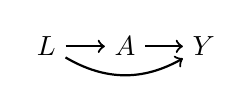
\begin{tikzpicture}
\node (l) at (0,0) {$L$};
\node (a) at (1,0) {$A$};
\node (y) at (2,0) {$Y$};
\draw[->, thick] (l) -- (a);
\draw[->, thick] (l) to[bend right] (y);
\draw[->, thick] (a) -- (y);
\end{tikzpicture}
\end{center}
where data are generated by the following data generating process.

For $i = 1,\dots,n$
\begin{align}
    L_i &\sim\text{Bernoulli}(0.5) &\text{binary confounder} \\
    \vec\lambda_i &= \begin{cases}
    \left(\begin{matrix}\frac{2}{3} & \frac{1}{6} & \frac{1}{6}\end{matrix}\right)^T &\text{if }A_i = 0 \\
    \left(\begin{matrix}\frac{1}{6} & \frac{1}{6} & \frac{2}{3}\end{matrix}\right)^T &\text{if }A_i = 1
    \end{cases} &\text{probability of treatment values \{1,2,3\}}\label{eq:pi} \\
    A_i &\sim\text{Multinomial}\left(\vec\lambda_i\right) &\text{categorical treatment} \\
    \mu_i &= L_i + A_i + L_iA_i &\text{outcome mean} \label{eq:mu} \\
    Y_i &\sim\text{Normal}(\text{Mean} = \mu_i, \text{SD} = 5) &\text{continuous outcome}
\end{align}

Eq~\ref{eq:pi} is designed so that $L$ is imbalanced across the treatment.
\begin{itemize}
    \item Much higher probability mass on $A = 1$ when $L = 0$
    \item Much higher probability mass on $A = 3$ when $L - 1$
\end{itemize}
Eq~\ref{eq:mu} is designed so that $L$ directly affects the outcome, and so that the response surface is interactive.

The figure below visualizes the response surface.

\begin{center}
    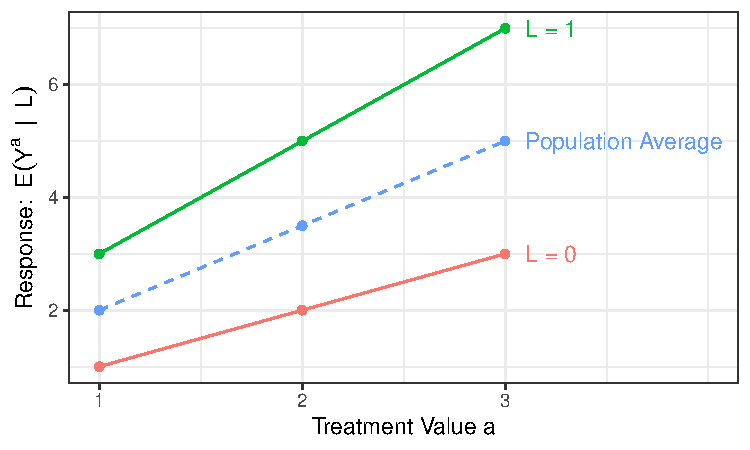
\includegraphics[width = 4in]{figures/dgp.pdf}
\end{center}

Although a lines are shown, the data are discrete with only treatment values $A \in \{1,2,3\}$.

You will submit
\begin{itemize}
    \item A PDF with your answers
    \item A file with your code, or have code embedded within the PDF above
\end{itemize}\newpage

\section{(25 points) Material covered Tuesday}
Part 1 is about the \textbf{inverse probability weighting}.

\begin{enumerate}
    \item (5 points) Nonparametrically estimate each unit's generalized propensity score: $\hat\pi_i = \hat\P(A = a_i\mid \vec{L} = \vec\ell_i)$. To facilitate grading, report the estimated propensity score for the first unit in the dataset.
    \item (5 points) Create the inverse probability weight $\hat{w}_i = \frac{1}{\hat\pi_i}$ for each unit. To facilitate grading, report the estimated weight for the first unit in the dataset.
    \item (10 points) For each treatment value $a = \{1,2,3\}$, estimate the population-average response $\E(Y^a)$ by inverse probability weighting. Report the three estimates.
    \item (5 points) Summarize the population-average response curve estimate in a graph.
\end{enumerate}

\section{(25 points) Material covered Thursday}
Part 2 is about the \textbf{marginal structural models}.

In Part (1) we estimated entirely by treatment modeling with no assumptions about the shape of the response surface. In the parametric $g$-formula of prior weeks, we assumed a functional form for the entire response surface $\E(Y\mid A,\vec{L})$. A marginal structural model is between these extremes: we make assumptions about the form of the population-average treatment response $\E(Y^a)$ marginalized over the population distribution of confounders. In this part, we will assume a linear marginal structural model,
\begin{equation}
    \E(Y^a) = \alpha + \beta a \label{eq:msm}
\end{equation}
Note that the marginal structural model (Eq~\ref{eq:msm}) is a model for the mean of potential outcomes rather than factual outcomes ($\E(Y^a)$ instead of $\E(Y\mid A = a)$), so it is not a standard OLS equation and must be estimated with inverse probability weighting.

\begin{enumerate}
    \item (15 points) Estimate the marginal structural model using OLS weighted by the inverse probability of treatment weights from 1.2. Report the coefficient estimate $\hat\beta$.
    \item (5 points) Produce a graph summarizing the population-average response curve as estimated by both methods (IPW and MSM-IPW).
    \item (5 points) Comment on the differences between the two estimates. Why might we prefer one or the other?
\end{enumerate}

\end{document}

